\subsection{Energiespeicher}
	Das Ziel des Energiespeichers ist es m�glichst viel Energie in einem m�glichst kleinen Volumen zu speichern und diese effizient aufzunehmen und abzugeben. Der Aufbau dieser Batterien besteht meistens aus zwei unterschiedlichen Elektroden und aus einem dazwischen befindlichen Elektrolyt. Die Spannung einer solchen Zelle h�ngt von  der Differenz der Elektronegativit�t der beiden Elektroden ab. Die wichtigsten Eckdaten eines Akkus sind seine Spannung in V, seine Kapazit�t in Wh und die Endlade- und Laderate in C($\frac{Entladestrom}{Kapazit\ddot{a}t}$). Die meisten Akkus bestehen aus mehreren Zellen die in Serie oder parallel geschalten sind, um entweder Spannung oder Kapazit�t zu erh�hen. Daraus entstehen Bezeichnungen f�r Akkus wie zum Beispiel 4S2P, welches f�r 4 Serielle Zellen, 2 mal parllel geschalten steht. 
	
	\begin{figure}[H]
		\centering
		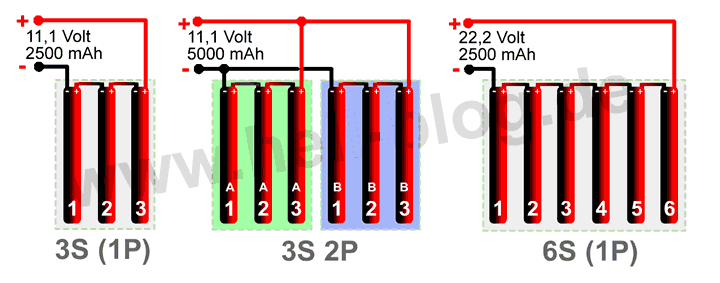
\includegraphics[scale=0.4]{./3_Stand_der_Technik/Abbildungen/Akku_3}
		\caption{Serien- und Parallelschaltung von Akkuzellen\cite{heliplanet.com2024}}
	\end{figure}
	
	Bei Akkus mit mehreren Zellen ist es wichtig darauf zu achten, dass die Zellspannung der unterschiedlichen Zellen nicht variiert. Wenn eine Zelle voll geladen und eine zweite komplett entladen ist, wirkt der Akku anhand der gesamten Akku-Spannung als zur H�lfte geladen. Wenn jedoch eine Entladestrom flie�t, wird eine Zelle unter ihre Abschaltspannung geladen, was zum Schaden der Zelle oder wie im Fall von Lithium Zellen auch zum Brand oder zur Explosion f�hren kann. Um diesem Problem vorzubeugen sind auf Akkus mit mehreren Zellen Balance Stecker angebracht, mithilfe von welchen die einzelnen Zellspannungen gemessen und ausgeglichen werden k�nnen. Der Ausgleich der Zellspannungen findet meistens bei jedem Ladevorgang statt.
	
	\begin{figure}[H]
		\centering
		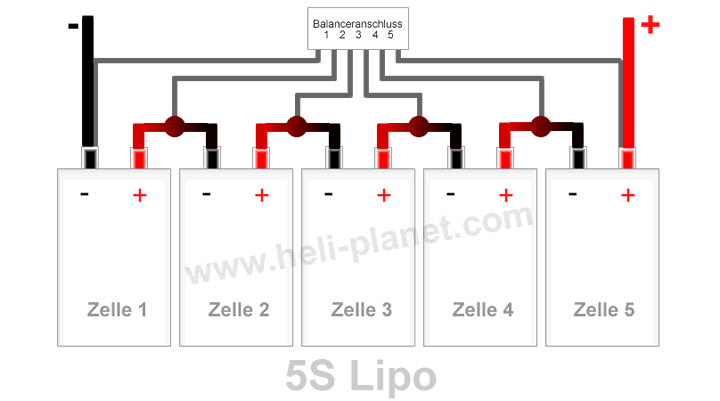
\includegraphics[scale=0.5]{./3_Stand_der_Technik/Abbildungen/Akku_4}
		\caption{Balance-Stecker\cite{heliplanet.com2024}}
	\end{figure}

	\subsubsection{Alkali-Mangan-Zelle(AlMn)}
		Alkali-Mangan Batterien sind das am h�ufigsten verwendete Batteriesystem, sie �berzeugen vorallem mit ihrer hohen Verf�gbarkeit und g�nstigen Herstellung. Sie bieten auch eine recht hohe Energiedichte. Sie haben auch eine lange Haltbarkeit und ein niedrige Selbstentladung. Zu den Nachteilen z�hlt die geringe Entladerate, die oft unter 0,1C liegt und die begrenzte Wideraufladbarkeit. Die h�ufigste Form dieser Batterie ist die AA und AAA Batterie.\cite{Fricke2007} Die Zellspannung einer Alkali-Mangan-Zelle betr�gt 1,5V.
		
		\begin{figure}[H]
			\centering
			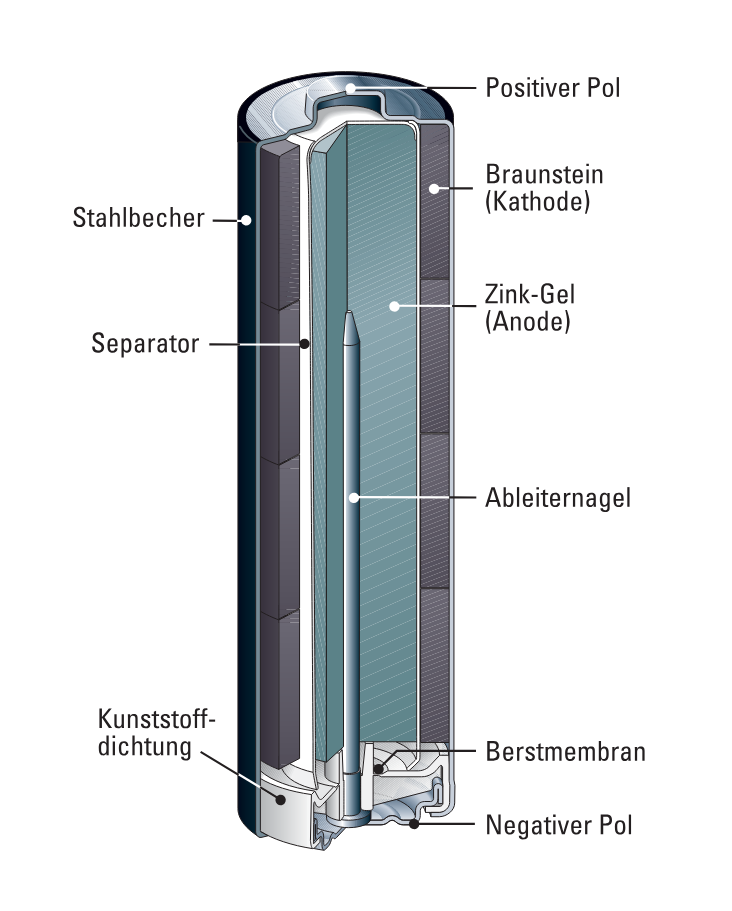
\includegraphics[scale=0.5]{./3_Stand_der_Technik/Abbildungen/Akku_1}
			\caption{Alkali-Mangan-Zelle\cite{Fricke2007}}
		\end{figure}
	
	\subsubsection{Silberoxid-Zelle(AgO)}
		Silberoxid Zellen werden vorwiergend f�r sehr kleine Knopfzellen verwendet, wo hohe Energiedichte ebenso wie geringes Volumen hohe Priorit�t hat. Ihr Aufbau ist sehr �hnlich zu dem der Alkali-Mangan-Zelle. Da die Materialien in gro�en Mengen sehr teuer sind, wird sie meistens nur in geringen Gr��en verwendet. Die Zellspannung einer Silberoxid-Zelle betr�gt 1,6V.\cite{Fricke2007} 
		
		\begin{figure}[H]
			\centering
			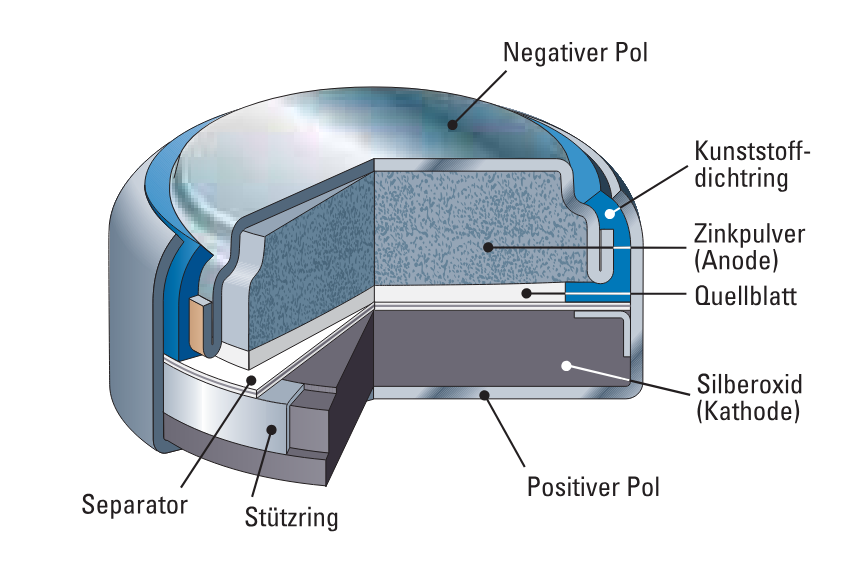
\includegraphics[scale=0.5]{./3_Stand_der_Technik/Abbildungen/Akku_2}
			\caption{Silberoxid-Zelle\cite{Fricke2007}}
		\end{figure}
	
	\subsubsection{Nickel-Cadmium-Zelle(NiCd)}
		Nicke-Cadmium-Zellen �berzeugen vorallem durch ihre hohe Belastbarkeit, Schnellladef�higkeit und K�lteresistenz. Sie haben jedoch einen relativ geringen Energieinhalt im Vergleich zu Lithium- oder Alkalisystemen. Ein ebenso gro�er Nachteil is das Auftreten des Memory-Effekts, wenn die Zelle vor dem Vollst�ndig Entladen wieder aufgeladen wird, k�nnen sich Kristalle bilden, die die Kapazit�t wesentlich verringern. Nickel-Cadmium-Zellen haben eine Zellspannung von 1,2V.
	
	\subsubsection{Nickel-Metallhybrid-Zelle(NiMH)}
	
	\subsubsection{Lithium-Ion-Zelle{Li-Ion}}
	
	\subsubsection{Lithium-Polymer-Zelle}